\documentclass{ltjsarticle}
%%%package読み込み
\usepackage{amsmath}
\usepackage{amssymb}
\usepackage{amsfonts}
\usepackage{mathtools}
\usepackage{bm}
% \usepackage{tikz} % ★消去: 代わりに graphicx 追加
% \usetikzlibrary{cd}
\usepackage{url}
\usepackage{graphicx} % ★追加: 図を挿入するため
\usepackage{float} % ★追加: 図の位置を制御するため
\usepackage{caption} % ★追加: 図のキャプションを柔軟に扱うため
%\usepackage{xcolor}
\usepackage{ascmac}
\usepackage{tcolorbox}
%\usepackage[dvipdfmx, setpagesize=false, bookmarks=true, bookmarksdepth=tocdepth, bookmarksnumbered=true, colorlinks=true, linkcolor=red]
\usepackage{hyperref}
\usepackage[version=4]{mhchem}
\usepackage{braket} % 追加した
\usepackage{booktabs}
\usepackage{bookmark}
%\usepackage[textwidth=45zw,lines=44]{geometry}
%\usepackage{pxjahyper}
%%%黒板太字
\newcommand{\N}{\mathbb{N}}
\newcommand{\Z}{\mathbb{Z}}
\newcommand{\Q}{\mathbb{Q}}
\newcommand{\R}{\mathbb{R}}
\newcommand{\C}{\mathbb{C}}
\newcommand{\F}{\mathbb{F}}
%%%約物
\newcommand{\abs}[1]{\left|#1\right|}
\newcommand{\lr}[1]{\left(#1\right)}
\newcommand{\st}{\; \mathrm{s.t.}\; }
\newcommand{\Ae}{\textrm{-a.e.}} 
%%%繰り返し
\newcommand{\pluss}[3]{#1_{#2}+\cdots+#1_{#3}}
\newcommand{\minuss}[3]{#1_{#2}-\cdots-#1_{#3}}
\newcommand{\timess}[3]{#1_{#2}\times\cdots\times #1_{#3}}
\newcommand{\leqs}[3]{#1_{#2}\leq\cdots\leq #1_{#3}}
\newcommand{\geqs}[3]{#1_{#2}\geq\cdots\geq #1_{#3}}
\newcommand{\opluss}[3]{#1_{#2}\oplus\cdots\oplus #1_{#3}}
\newcommand{\otimess}[3]{#1_{#2}\otimes\cdots\otimes #1_{#3}}
\newcommand{\commas}[3]{#1_{#2},\ldots,#1_{#3}}
%%%微分
\newcommand{\dx}[1]{\mathrm{d}#1}
\newcommand{\ddx}[1]{\frac{\mathrm{d}}{\mathrm{d}#1}}
\newcommand{\dydx}[2]{\frac{\mathrm{d}#1}{\mathrm{d}#2}}
\newcommand{\dydxn}[3]{\frac{\mathrm{d}^{#3}#1}{\mathrm{d}#2^{#3}}}
\newcommand{\del}[2]{\frac{\partial#1}{\partial#2}}
\newcommand{\dell}[2]{\frac{\partial^2#1}{{\partial#2}^2}}
\newcommand{\deln}[3]{\frac{\partial^{#3}#1}{{\partial#2}^{#3}}}
%%%
%%%演算子
%log type
\let\Re\relax
\DeclareMathOperator{\Re}{Re}
\let\Im\relax
\DeclareMathOperator{\Im}{Im}
\DeclareMathOperator{\sgn}{sgn}
\DeclareMathOperator{\sign}{sign}
\DeclareMathOperator{\Supp}{Supp}
\DeclareMathOperator{\tr}{tr}
\DeclareMathOperator{\Tr}{Tr}
\DeclareMathOperator{\Det}{Det}
\DeclareMathOperator{\Log}{Log}
\DeclareMathOperator{\rank}{rank}
\DeclareMathOperator{\diag}{diag}
\DeclareMathOperator{\corank}{corank}
\DeclareMathOperator{\Res}{Res}
\DeclareMathOperator{\Ker}{Ker}
\DeclareMathOperator{\coker}{coker}
\DeclareMathOperator{\Coker}{Coker}
\DeclareMathOperator{\Var}{Var}
\DeclareMathOperator{\Cov}{Cov}
\DeclareMathOperator{\sech}{sech}
\DeclareMathOperator{\csch}{csch}
\DeclareMathOperator{\arcsec}{arcsec}
\DeclareMathOperator{\arccot}{arccot}
\DeclareMathOperator{\arccsc}{arccsc}
\DeclareMathOperator{\arccosh}{arccosh}
\DeclareMathOperator{\arcsinh}{arcsinh}
\DeclareMathOperator{\arctanh}{arctanh}
\DeclareMathOperator{\arcsech}{arcsech}
\DeclareMathOperator{\arccsch}{arccsch}
\DeclareMathOperator{\arccoth}{arccoth}
\DeclareMathOperator{\grad}{grad}
\let\div\relax
\DeclareMathOperator{\div}{div}
\DeclareMathOperator{\rot}{rot}
%\DeclareMathOperator{\GL}{GL} % ★消去 : ここから↓
%\DeclareMathOperator{\SL}{SL}
%\DeclareMathOperator{\Sym}{Sym}
%\DeclareMathOperator{\Aut}{Aut}
%\DeclareMathOperator{\Inn}{Inn}
%\DeclareMathOperator{\Out}{Out}
%\DeclareMathOperator{\id}{id}
%\DeclareMathOperator{\pr}{pr}
%\DeclareMathOperator{\supp}{supp}
%\DeclareMathOperator{\diam}{diam}
%\DeclareMathOperator{\End}{End}
%\DeclareMathOperator{\Cl}{Cl}
%\DeclareMathOperator{\Hom}{Hom} % ★消去 : ここまで↑
%limit type
\DeclareMathOperator*{\argmin}{arg~min}
\DeclareMathOperator*{\argmax}{arg~max}
%%%
%%%定理
\usepackage{amsthm}
\theoremstyle{definition}
\newtheorem{lem}{補題}
\newtheorem*{lem*}{補題}
\newtheorem{prf}{証明}
\newtheorem*{prf*}{証明}
\newtheorem*{ex*}{Example}
\newtheorem*{rem*}{Remark}
\newenvironment{prb}[1]%
{\begin{itembox}[l]{\textbf{問題 #1}}}%
{\end{itembox}}
\newenvironment{sol}[2]%
{\setcounter{lem}{0}
\setcounter{prf}{0}
\par\noindent\textbf{解答 #1} (#2)\par}%
{\par\normalfont}

\renewcommand{\refname}{Reference}


%%%%%%%%%%%%%%%%%%%%%
\numberwithin{equation}{section}
%%%%%%%%%%%%%%%%%%%%%%

\newcounter{boxeddefcounter}
\newenvironment{problem}
{\refstepcounter{boxeddefcounter}\begin{itembox}[l]{問\theboxeddefcounter}}
{\end{itembox}}

%\usepackage[hang,small,bf]{caption}
%\usepackage[subrefformat=parens]{subcaption}
\captionsetup{compatibility=false}


\newcommand{\D}{^\circ\text{C}}
\newcommand{\ka}{\textasciitilde}


\pagestyle{myheadings}
\title{有機化学実験 文献調査}
\date{\today}
\author{Author: No.7 05253011 Fumiya Kashiwai / 柏井史哉}
\begin{document}
\maketitle
\markboth{Organic experiment Literature report No.7 05253011 Fumiya Kashiwai / 柏井史哉} {Organic experiment Literature report No.7 05253011 Fumiya Kashiwai / 柏井史哉}
%%ここまでタイトル
\section{化合物情報}
\begin{figure}[htbp]
\begin{center}
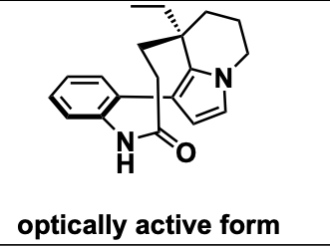
\includegraphics[width = 5 cm]{structure.png}
\caption{(-)- Rhazinilam の構造}
\label{default}
\end{center}
\end{figure}
CAS Registry Number: 36193-36-9

IUPAC名: Indolizino[8,1-ef][1]benzazonin-6(5H)-one

化合物名: (R) - Rhazinilam / (-)- Rhazinilam


\section{経路選択とその根拠}
反応スキームは以下に示したとおり、\cite{sugimoto_1}の手法を選択した。連続15 stepでoverallの収率が10\%程度である。また$ee > 99\%$であることが報告されている。
光学活性体の合成を行っている論文をReview論文\cite{Magnus}を参考に選抜し、そのうち高い$ee$で不斉合成を行っている上記の論文を選択した。
他の不斉合成法\cite{gau}は、13 step, 19\%と今回参考にした方法よりもステップ数が少なく、かつ収率が高いが、光学選択性が 92 : 8と劣る点と、独自に合成された複雑なキラル試薬を用いていることから除外した。
\cite{sugimoto_1}と同じ筆者による\cite{sugimoto_2}はキラルプール法によりD-アスパラギン酸から合成しており、特殊な試薬を用いていないため有望であるが、ステップ数が14 stepでほぼ変わらず、収率が7\%と落ちることから\cite{sugimoto_1}を選択することにした。

\section{スキーム}
次ページの図\ref{scheme}に示した。
\begin{figure}[htbp]
\begin{center}
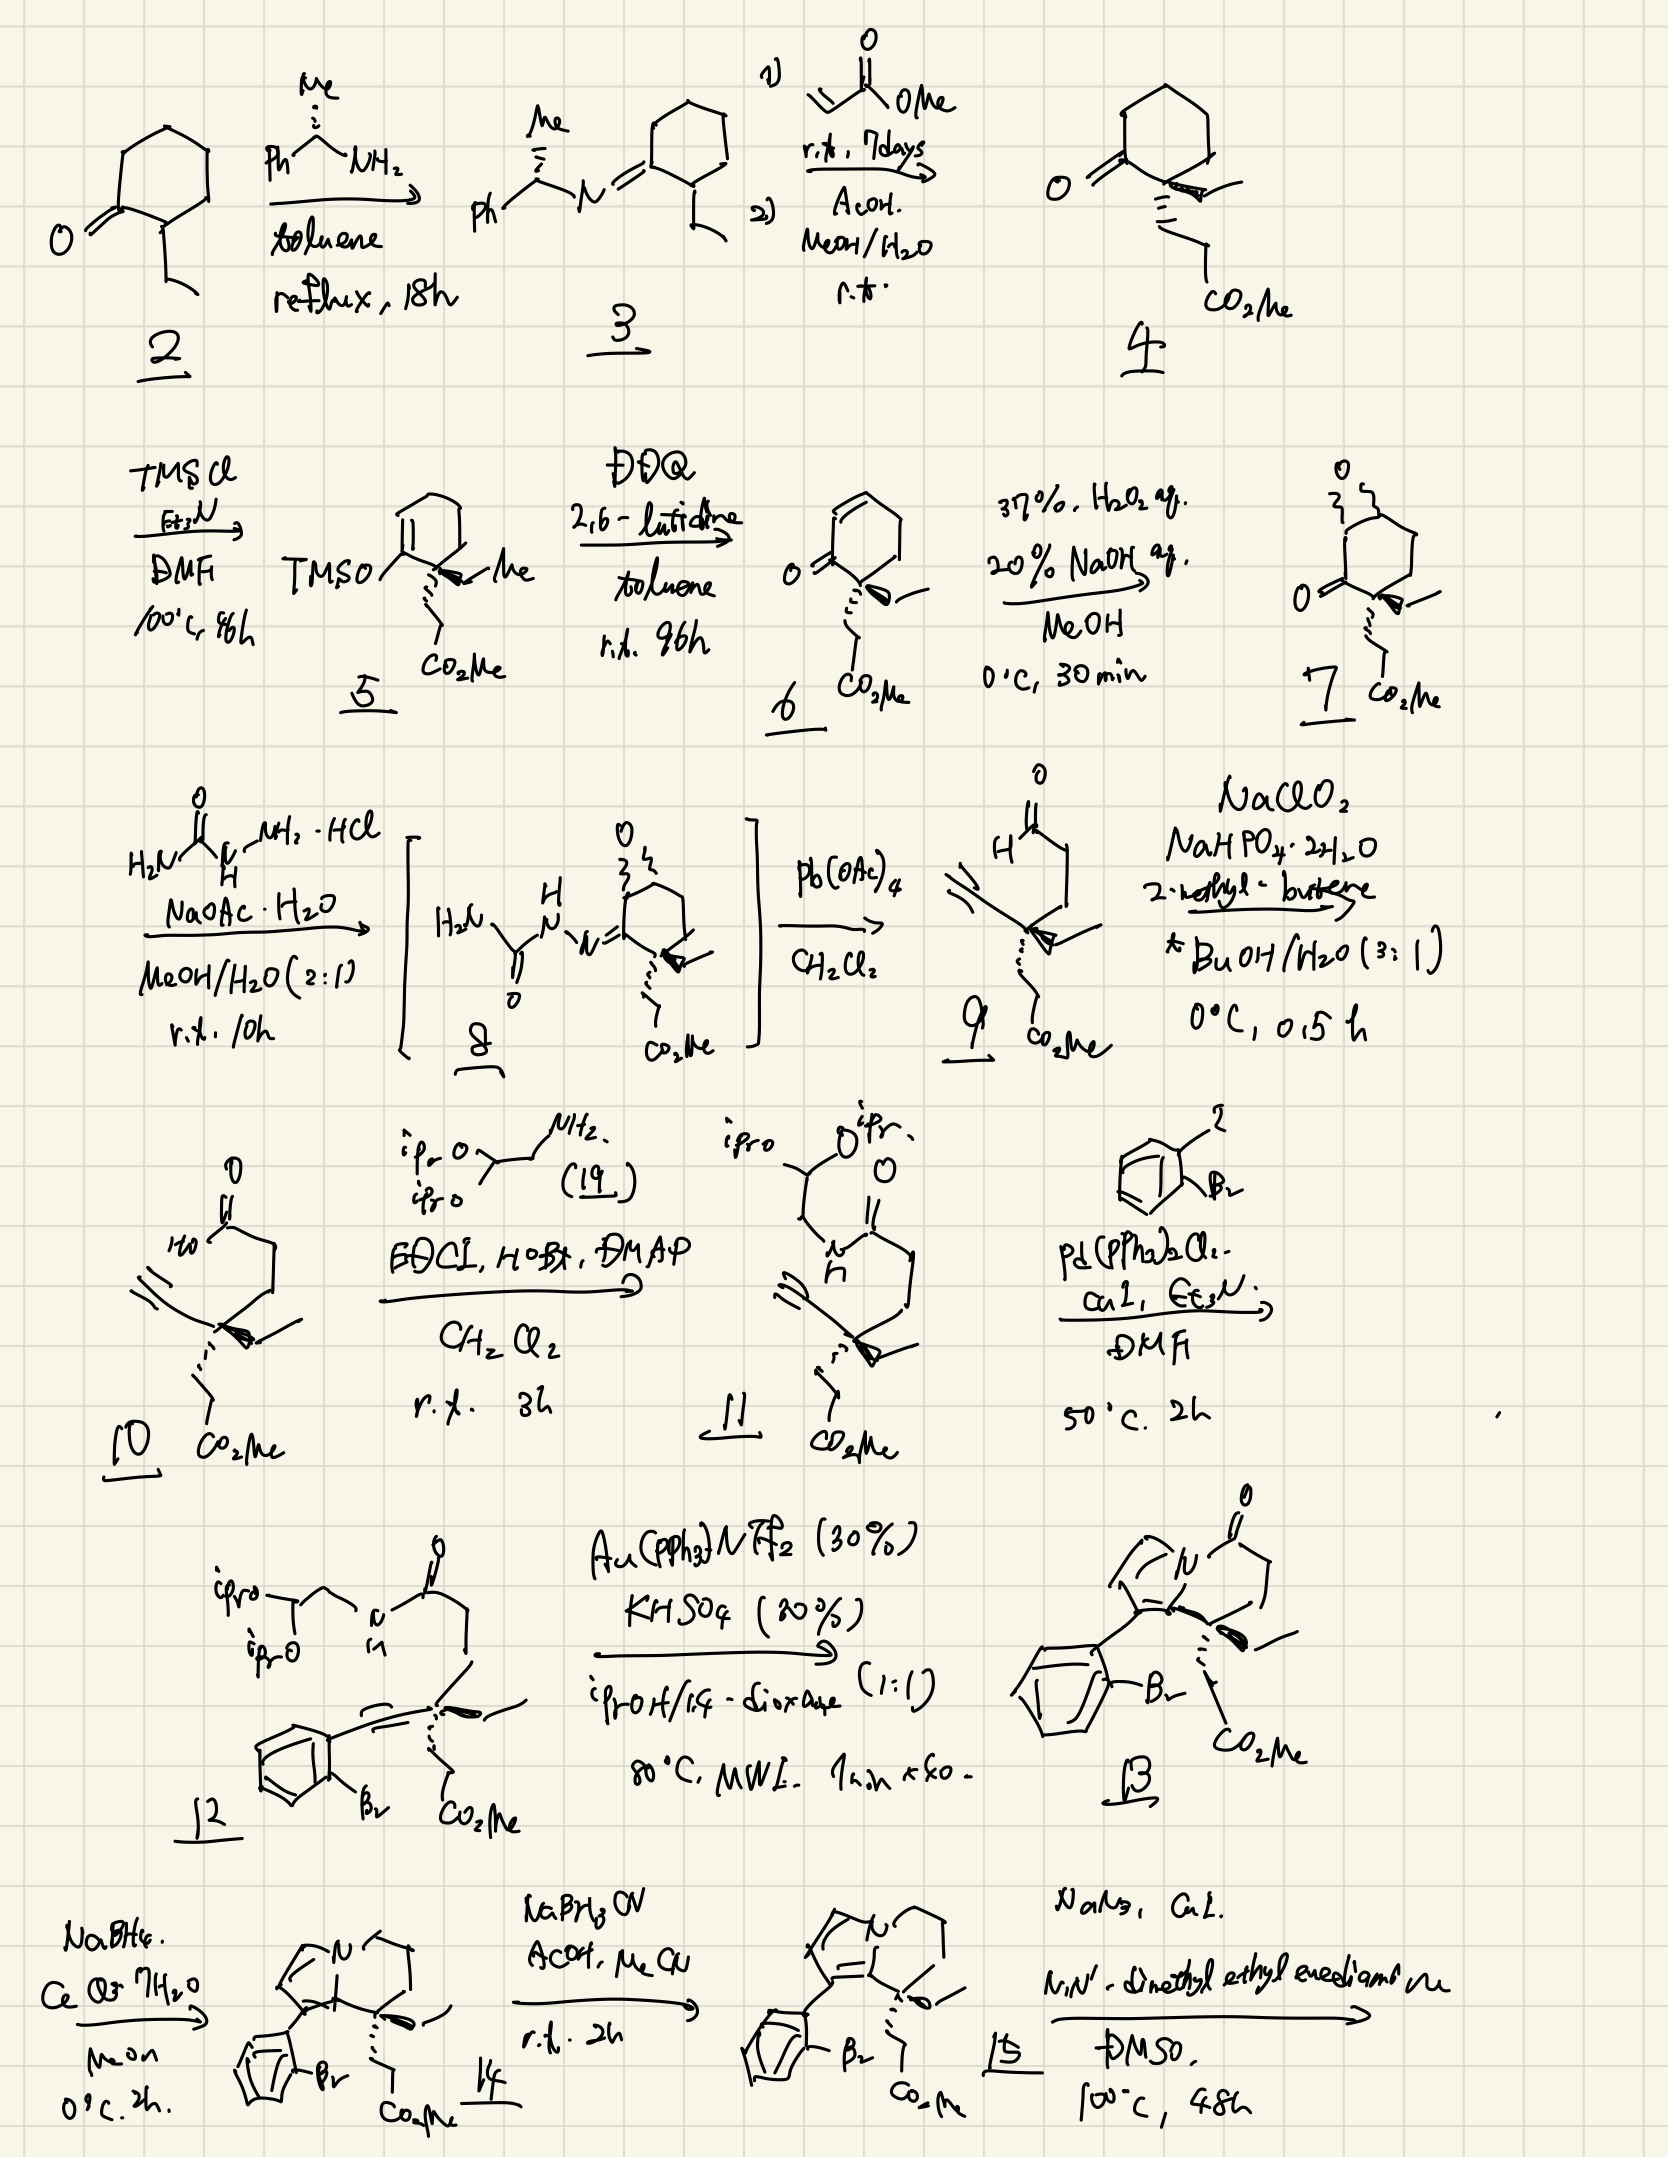
\includegraphics[width = 13 cm]{scheme1.jpg}
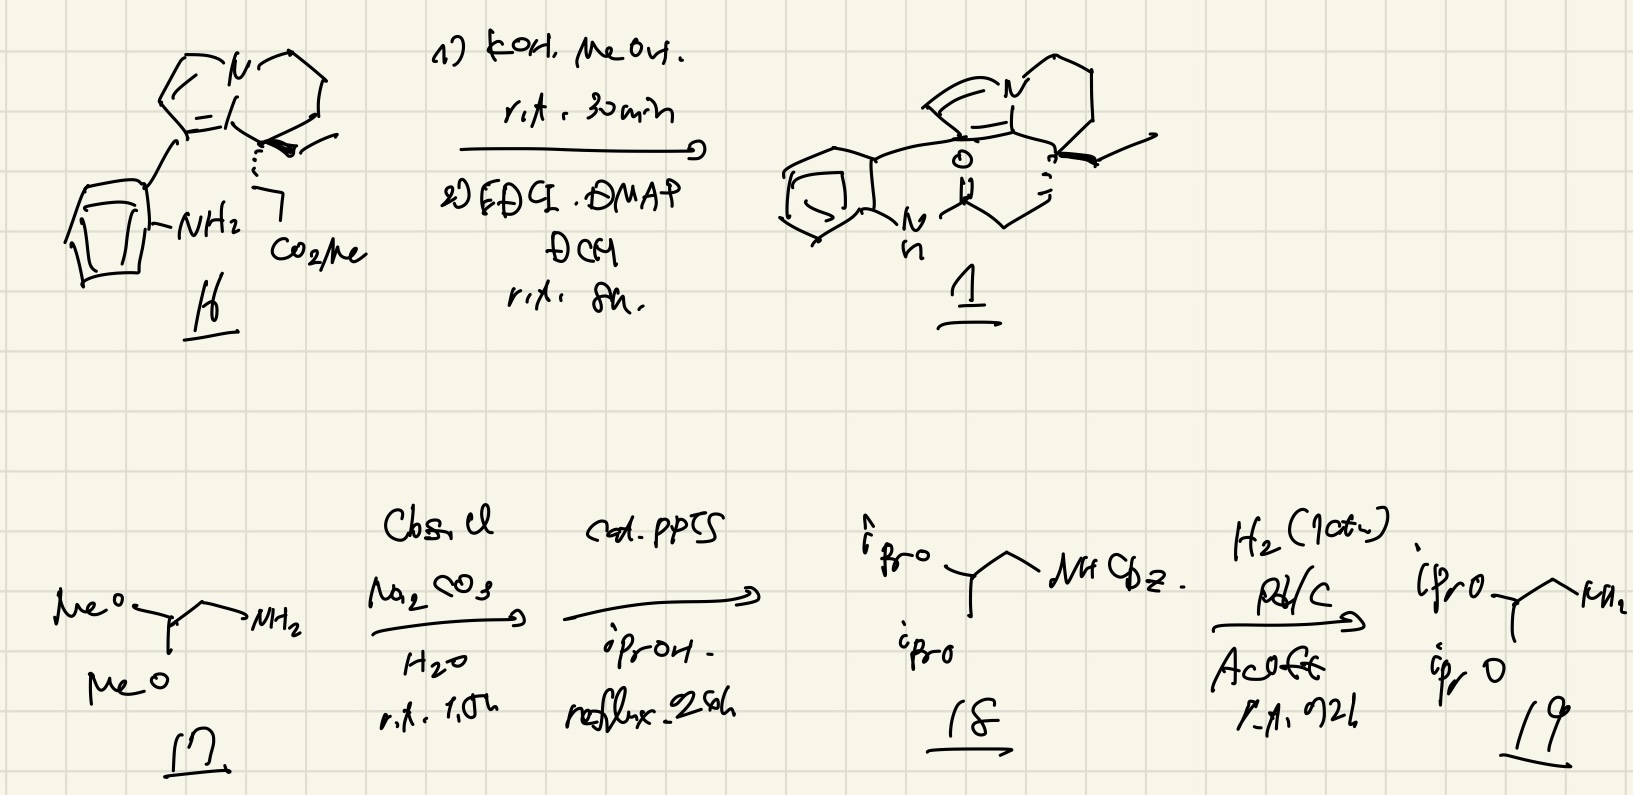
\includegraphics[width = 13 cm]{scheme2.jpg}
\caption{(-)- Rhazinilam の合成経路}
\label{scheme}
\end{center}
\end{figure}


\section{実験手順}
\subsection{注釈}
・分量の記載のない試薬類は、元論文に記載のなかった部分であり、適量を用いると考えられる。

\begin{table}[htp]
\caption{略称の定義}
\begin{center}
\begin{tabular}{cc }
\toprule
略称 & 正式名称 \\
\midrule
Brine & 飽和食塩水 \\
CbzCI & Chloroformic Acid Benzyl Ester\\
DCM & Dichloromethane \\
DDQ & 2,3-Dichloro-5,6-dicyano-p-benzoquinone \\
DMAP & 4-Dimethylaminopyridine\\
DMF & \textit{N,N-}dimethylformamide \\
EDCI & 1-(3-Dimethylaminopropyl)-3-ethylcarbodiimide Hydrochloride\\
HOBt & 1-Hydroxybenzotriazole Monohydrate \\
PPTS & Pyridinium \textit{p-}toluenesulfonate \\
\bottomrule
\end{tabular}
\end{center}
\label{default}
\end{table}%

\subsection{\textbf{2} → \textbf{4}}
化合物\textbf{2} (7.00  g, 55.2 mmol) と toluene (21 mL) をフラスコに量り取り、Dean-Stark装置をセットする。
(S)-1-Phenylethylamine (8.4 mL , 66.2 mmol) を加え、18 h加熱還流する。
冷却後、減圧下で濃縮し、黄色い油状の粗精製物\textbf{3}を得る。

粗精製物\textbf{3}にmethyl acetate (7.97 mL, 88.3 mmol) を加え、室温で7 days撹拌する。
過剰量のmethyl acetate を減圧下で除去したのち、\ce{AcOH} (5 mL) 、\ce{H2O} (20 mL)、\ce{MeOH} (10 mL) を加え、室温で3 h撹拌したのち、\ce{NaCl}で飽和させて、\ce{Et2O}で3回抽出する。有機層を合わせて1M \ce{HCl}\textit{aq.}、飽和\ce{NaHCO3}\textit{aq.}、Brineで洗浄し、\ce{Na2SO4}で乾燥、濾過ののち減圧下で濃縮する。カラム精製 (\ce{hexane/AcOEt}, 8:2)により無色油状の化合物\textbf{4} (9.72 g, 45.8 mmol, 83\%)を得る。

\subsection{\textbf{4} → \textbf{6}}
化合物\textbf{4} (9.71  g, 45.8 mmol)、\ce{DMF} (46 mL) をフラスコに量り取る。
\ce{Et3N} (31.7 mL, 229 mmol) 、\ce{TMSCl} (23.2 mL, 183 mmol)を室温で加え、100$\D$で46 h撹拌したのち、hexaneとwaterで希釈する。
水層をhexaneで3回抽出する。有機層を合わせてBrineによる洗浄、\ce{Na2SO4}による乾燥、濾過、減圧下で濃縮することで粗精製物\textbf{5}を得る。これ以上の精製操作はせずに次の反応に用いる。

粗精製物\textbf{5}をフラスコに移し、toluene (140 mL) を量り取る。
DDQ (11.4 g,  63.0 mmol)、2,6-lutidine (9.12 mL, 63.0 mmol)を室温で加え、室温で48 h激しく撹拌したのち、DDQ (7.63 g, 20.9 mmol)、2,6-lutidine (6.11mL, 20.9 mmol) をさらに加え、さらに48 h撹拌する。\ce{AcOEt}で希釈し、silica padで濾過する。黒色固体を\ce{AcOEt}で繰り返し洗浄し、減圧下で濃縮する。\\
カラム精製 (\ce{hexane/AcOEt}, 9:1 - 7:3)により無色油状の化合物\textbf{6} (7.73 g, 36.6 mmol, 80\%) を得る。


\subsection{\textbf{6} → \textbf{7}}
化合物\textbf{6} (7.70  g, 36.5 mmol)、MeOH (37 mL) をフラスコに量り取る。
20\% \ce{NaOH}\textit{aq.} (0.70 mL, 3.72 mmol)、37\% \ce{H2O2}\textit{aq.} (18.1 mL, 193 mmol) の順に0$\D$で加え、30 min撹拌したのち、\ce{AcOH}を加えて反応を停止する。
反応溶液をBrineに注ぎ、\ce{Et2O}を用いて3回抽出する。有機層を合わせて\ce{NaHSO3}による乾燥、濾過ののち減圧下で濃縮する。
カラム精製 (hexane/AcOEt, 8:2) により化合物\textbf{7} (7.59 g, 33.6 mmol, 92\%)を得る。


\subsection{\textbf{7} → \textbf{10}}
化合物\textbf{7} (7.57 g, 33.5 mmol)、water (50 mL)、\ce{MeOH} (100 mL) をフラスコに量り取る。
semicarbazide hydrochloride (29.6 g, 265 mmol)、\ce{NaOAc} (5.71 g, 69.6 mmol) を室温で加え、室温で10 h撹拌する。減圧下で\ce{MeOH}を除去し、DCMを用いて3回抽出する。有機層を合わせてBrineによる洗浄、\ce{NaHSO3}による乾燥、濾過ののち減圧下で濃縮する。
溶媒の留去ののち、白色固体として粗精製物\textbf{8}を得る。これ以上の精製操作はせずに次の反応に用いる。

粗精製物\textbf{8}をフラスコに移し、DCM (170 mL) を量り取る。
\ce{Pb(OAc)4} (18.0 g, 40.7 mmol) を-10$\D$で加え、2 h撹拌したのち、Celite padにより濾過、減圧下で濃縮して黄色油状の粗精製物\textbf{9} を得る。これ以上の精製操作はせずに次の反応に用いる。

粗精製物\textbf{9}をフラスコに移し、water (30 mL)、\textit{t-}\ce{BuOH} (90 mL)を量り取る。
2-methy-2-butene (35.6 mL, 336 mmol)、\ce{NaH2PO4*2H2O} (10.6 g, 67.7 mmol)、\ce{NaClO4} (6.20 g, 68.5 mmol) を0$\D$で加え、室温で2 h撹拌したのち、4 M HCl\textit{aq.}で反応を停止する。水層をDCMを用いて5回抽出する。有機層を合わせてBrineによる洗浄、\ce{Na2SO3}による乾燥、濾過ののち減圧下で濃縮する。
カラム精製 (hexane/AcOEt, 3:7) により化合物\textbf{10} (4.54 g, 20.1 mmol, 60\%)を得る。

\subsection{\textbf{10} → \textbf{11}}
化合物\textbf{10}  (4.52  g, 20.0 mmol)、\ce{DCM} (200 mL)をフラスコに量り取る。
EDCI (11.5 g, 60.0 mmol) 、\ce{HOBt} (4.89 g, 40.0 mmol)、DMAP (hogehoge) を加え、次いで化合物\textbf{19} (3.00 g, 30.0 mmol) を0$\D$で加える。室温で3 h撹拌したのち、飽和\ce{NH4Cl}\textit{aq.} を加えて停止する。DCMを用いて3回抽出する。有機層を合わせてBrineによる洗浄、\ce{NaHSO3}による乾燥、濾過ののち減圧下で濃縮する。
カラム精製 (hexane/\ce{AcOEt}, 3:7) により、無色油状の化合物\textbf{11} (5.52 g, 17.8 mmol, 79\%)を得る。

\subsection{\textbf{11} → \textbf{12}}
化合物\textbf{11} (5.43  g, 17.5 mmol)、DMF (30 mL)をフラスコに量り取る。
2-bromoiodobenzene (2.7 mL, 21 mmol)、\ce{Et3N} (7.2 mL, 53 mmol)、\ce{CuI} (215 mg ,1.13 mmol)、\ce{Pd(PPh3)2Cl2} (368 mg , 0.53 mmol)を室温で加え、50$\D$で2 h撹拌したのち\ce{AcOEt}で希釈し、\ce{NH4Cl}\textit{aq.}を加えて停止する。\ce{AcOEt}を用いて3回抽出する。有機層を合わせてBrineによる洗浄、\ce{MgSO4}による乾燥、Celite padによる濾過ののち減圧下で濃縮する。
カラム精製(hexane/AcOEt, 3:7) により、無色油状の化合物\textbf{12} (6.08 g, 15.1 mmol, 86\%)を得る。

\subsection{\textbf{12} → \textbf{13}}
化合物\textbf{12} (6.00  g, 14.9 mmol)、1,4-dioxane (150 mL) をフラスコに量り取る。
\ce{Au(PPh3)NTs2} (3.30 g, 4.47 mmol) と \ce{KHSO4} (0.63 g, 4.47 mmol) を室温で加え、80$\D$でマイクロ波照射60 sec$\times$40回 (90秒インターバル) で反応させたのち飽和\ce{NaHCO3}\textit{aq.}を加えて停止する。反応溶液全体をDCMで3回抽出する。有機層を合わせてBrineによる洗浄、\ce{Na2SO3}による乾燥、濾過ののち減圧下で濃縮する。
分取TLC (hexane/AcOEt, 7:3) で精製し、無色油状の化合物\textbf{13} (3.83 g, 9.69 mmol, 65\%)を得る。

\subsection{\textbf{13} → \textbf{15}}
化合物\textbf{13}  (3.55  g, 9.00 mmol)、MeOH (36 mL)をフラスコに量り取る。
0$\D$で\ce{NaBH4} (670 mg, 18.0 mmol )、\ce{CeCl3*7H2O} (7.25 g , 18.0 mmol) の順に加え、2 h撹拌したのち、飽和\ce{NH4Cl}\textit{aq.}を加えて停止する。反応溶液全体をDCMで3回抽出する。有機層を合わせてBrineによる洗浄、\ce{Na2SO3}による乾燥、濾過ののち減圧下で濃縮する。茶色油状の粗精製物\textbf{14} を得る。これ以上の精製操作はせずに次の反応に用いる。

得られた粗精製物\textbf{14}をフラスコに移し、\ce{AcOH} (4.2 mL)、 MeCN(42 mL) を量り取る。
室温で\ce{NaBH3CN} (5.61 g, 90.0 mmol) を加え、2 h撹拌したのち、飽和\ce{NaHCO3}\textit{aq.}を加えて停止する。反応溶液全体をDCMで3回抽出する。有機層を合わせてBrineによる洗浄、\ce{NaHSO3}による乾燥、濾過ののち減圧下で濃縮する。
分取TLC (\ce{AcOEt}) で精製し、無色油状の化合物\textbf{15} (2.81 g, 7.20 mmol, 80\%) を得る。

\subsection{\textbf{15} → \textbf{16}}
化合物\textbf{15}  (2.73 g, 7.00 mmol)、\ce{NaN3} (2.28 g, 35.0 mmol)、N,N’-dimethylethylenediamine (2.28 mL, 21.0 mmol)、DMSO (14 mL) をフラスコに量り取る。
\ce{CuI} (2.67 g, 14.0 mmol) を室温で加え、真空にしアルゴン置換する。アルゴン雰囲気下48 h、100$\D$で撹拌したのち、飽和\ce{NH4Cl}\textit{aq.} を加えて停止する。反応溶液全体をDCMで5回抽出する。有機層を合わせてBrineによる洗浄、\ce{Na2SO3}による乾燥、Celite板による濾過ののち減圧下で濃縮する。
分取TLC (\ce{AcOEt}) で精製し、無色油状の化合物\textbf{16} (1.47 g, 4.48 mmol, 64\%) を得る。

\subsection{\textbf{16} → \textbf{1}}
化合物\textbf{16}  (1.46 g, 4.46 mmol)、粉末状の\ce{KOH} (250 g, 4.5 mol)、および\ce{MeOH} (400 mL) を0$\D$でフラスコに量り取る。
室温で30 min攪拌したのち、0$\D$で4 M \ce{HCl}\textit{aq.}を加えて停止する。
生成物をDCMで5回抽出し、合わせた有機層を\ce{Na2SO4}で乾燥、濾過、減圧下で濃縮して茶色油状物を得る。これ以上の精製操作はせずに次の反応に用いる。
褐色の油状粗精製物をフラスコに移し、EDCI (1.28 g, 6.77 mmol)、HOBt (1.03 g, 6.77 mmol)、および DCM (640 mL) を0$\D$でフラスコに量り取る。
室温で8 h攪拌したのち、飽和\ce{NH4Cl}\textit{aq.}を加えて停止する。
反応溶液をDCMで5回抽出し、合わせた有機層を\ce{Na2SO4}で乾燥、濾過、する。反応溶液を\ce{AcOEt}で3回抽出し、合わせた有機層を\ce{Na2SO4}で乾燥、濾過、減圧下で濃縮する。
分取TLC (\ce{AcOEt}) で精製し、白色固体として化合物\textbf{1}を (1.00 g, 3.39 mmol, 76\%)得る。

\subsection{\textbf{17} → \textbf{18}}
化合物\textbf{17}  (7.22 mL, 65.0 mmol)、\ce{H2O} (220 mL) をフラスコに量り取る。
\ce{Na2CO3} (8.31 g, 78.4 mmol)、\ce{CbzCl} (11.2 mL, 75.8 mmol)を0$\D$で加え、室温で1.5 h撹拌したのち、飽和\ce{NaHCO3}\textit{aq.}で反応を停止する。反応溶液を\ce{AcOEt}で3回抽出し、無色油状の粗精製物を得る。これ以上の精製操作はせずに次の反応に用いる。
粗精製物をフラスコに移し、\textit{i-}\ce{PrOH} (220 mL)、PPTS (1.64 g, 6.53 mmol) を室温でフラスコに量りとり、100$\D$で24 h撹拌したのち、飽和\ce{NaHCO3}\textit{aq.}で反応を停止する。反応溶液を\ce{AcOEt}で3回抽出し、合わせた有機層を\ce{Na2SO4}で乾燥、濾過、減圧下で濃縮する。
カラム精製 (hexane/AcOEt, 8:2) により無色油状の化合物\textbf{18} (14.8 g, 50.1 mmol, 77\%) を得る。

\subsection{\textbf{18} → \textbf{19}}
化合物\textbf{18} (14.8  g, 50.0 mmol)、\ce{Pd/C} (Pd : 10\%, 2.47 g, 2.31 mmol)、\ce{AcOEt} (75 mL) をフラスコに量り取る。
\ce{H2} (1 atm) 雰囲気下、室温で12 h撹拌する。
 Celite板を用いて濾過したのち減圧下で濃縮し、黄色油状の化合物\textbf{19} (3.35 g, 33.5 mmol, 67\%) を得る。


%%参考文献
\begin{thebibliography}{99}
\bibitem{sugimoto_1}
Sugimoto, Kenji; Toyoshima, Kazuki; Nonaka, Shiori; Kotaki, Kenta; Ueda, Hirofumi; Tokuyama, Hidetoshi. Protecting-Group-Free Total Synthesis of (-)-Rhazinilam and (-)-Rhazinicine using a Gold-Catalyzed Cascade Cyclization. Angewandte Chemie, International Edition 52(28), 7168-7171 (2013).
\bibitem{Magnus}
Magnus Pfaffenbach, Tanja Gaich. The Rhazinilam-Leuconoxine-Mersicarpine Triad of Monoterpenoid Indole Alkaloids. The alkaloids: Chemistry and Biology, 77, 1-84 (2017).
\bibitem{gau}
Gualtierotti, Jean-Baptiste; Pasche, Delphine; Wang, Qian; Zhu, Jieping. Phosphoric acid catalyzed desymmetrization of bicyclic bislactones bearing an all-carbon stereogenic center: Total syntheses of (-)-rhazinilam and (-)-leucomidine B. Angewandte Chemie, International Edition 53(37), 9926-9930 (2014).
\bibitem{sugimoto_2}
Sugimoto, Kenji; Miyakawa, Yuta; Tokuyama, Hidetoshi. Total synthesis of (-)-rhazinilam using 1,3-dipolar cycloaddition of optically active munchnone intermediate. Tetrahedron 71(22), 3619-3624 (2015).
\end{thebibliography}

\end{document}